\documentclass{article}
\usepackage{amsmath}
\usepackage{amssymb}
\usepackage{graphicx}
\usepackage{float}
\usepackage{enumitem}
\usepackage{forest}
\usepackage{subcaption}
\usepackage{algorithm}
\usepackage{algpseudocode}

\begin{document}

\title{Homework 5}
\author{Manyara Bonface Baraka - mbaraka}
\date{\today}
\maketitle

\section{Gaussian Mixture Models [15 points]}

1-D Mixture Model Consider an exponential mixture model for a 1-D dataset $\{x_n\}$ with the density function
\[
p(x) = \sum_{k=1}^K \omega_k \text{Exp}(x|\mu_k),
\]
where $K$ is the number of mixture components, $\mu_k$ is the rate component, and $\omega_k$ is the mixture weight corresponding to the $k$-th component. The exponential distribution is given by
\[
\text{Exp}(x|\mu) = \mu \exp(-x\mu) \quad \text{for all } x \geq 0. \tag{1}
\]

We would like to derive the model parameters $(\omega_k, \mu_k)$ for all $k$ using the EM algorithm. Consider the hidden labels $z_n \in \{1, \ldots, K\}$ and indicator variables $r_{nk}$ that are 1 if $z_n = k$ and 0 otherwise. The complete log-likelihood (assuming base $e$ for the log) is then written as
\[
\sum_n \log p(x_n, z_n) = \sum_n \sum_{z_n=k} \left[\log p(z_n = k) + \log p(x_n|z_n = k)\right].
\]


\begin{enumerate}[label=(\alph*)]
    \item Write down and simplify the expression for the complete log-likelihood for the exponential mixture model described above. [5 points]
    \subsubsection*{Solution}
    We re-write it to:
    \[
    \sum_n \log p(x_n, z_n) = \sum_n \sum_{k=1}^K r_{nk} \left[\log p(z_n = k) + \log p(x_n|z_n = k)\right].
    \]
    Substitute:
    \begin{itemize}
        \item $p(z_n = k) = \omega_k$ for all $k$.
        \item $p(x_n|z_n = k) = \text{Exp}(x_n|\mu_k) = \mu_k \exp(-x_n\mu_k)$.
    \end{itemize}
    Thus, we have:
    \[
    \sum_n \log p(x_n, z_n) = \sum_n \sum_{k=1}^K r_{nk} \left[\log \omega_k + \log  \mu_k \exp(-x_n\mu_k)\right].
    \]
    \[
    \sum_n \log p(x_n, z_n) = \sum_n \sum_{k=1}^K r_{nk} \left[\log \omega_k + \log \mu_k - x_n\mu_k\right].
    \]

    Therefore, the complete log-likelihood can be simplified to:
    \[
    \sum_n \log p(x_n, z_n) = \sum_n \sum_{k=1}^K r_{nk} \left[\log \omega_k + \log \mu_k - x_n\mu_k\right].    
    \]
    % \begin{align*}
    %     \sum_{n} \log p(x_n, z_n) &= \sum_{k} \sum_{n} r_{nk} \left[\log \omega_k + \log \text{Exp}(x_n|\mu_k)\right] \\
    %     &= \sum_{k} \sum_{n} r_{nk} \left[\log \omega_k + \log \mu_k - x_n\mu_k\right].
    % \end{align*}

    \item Solve the M step of the EM algorithm and find $\mu_k$ for $k = 1, \ldots, K$ that maximizes the complete log-likelihood. [5 points]
    \subsubsection*{Solution}
    We need to maximize the expected complete log-likelihood with respect to $\mu_k$:\\
    For $\mu_k$: we need to find the value that maximizes:
    \[
    \sum_n \sum_{k=1}^K r_{nk} \left[\log \omega_k + \log \mu_k - x_n\mu_k\right].  
    \]

    To maximize this we do partial derivate and set it to zero:
    \[
    \frac{\partial}{\partial \mu_k} \sum_n \sum_{k=1}^K r_{nk} \left[\log \omega_k + \log \mu_k - x_n\mu_k\right] = 0.
    \]
    \[
    \sum_n r_{nk} \left[\frac{1}{\mu_k} - x_n\right] = 0.
    \]
    \[
    \sum_n r_{nk} x_n = \frac{1}{\mu_k} \sum_n r_{nk}.
    \]
    \[
    \mu_k = \frac{\sum_n r_{nk}}{\sum_n r_{nk} x_n}.
    \]




    % \begin{align*}
    % \frac{1}{\mu_k} \sum_{n} r_{nk} - \sum_{n} r_{nk} x_n &= 0 \\
    % \mu_k &= \frac{\sum_{n} r_{nk} x_n}{\sum_{n} r_{nk}}.
    % \end{align*}
    
    \item Now perform the E step, and write the equation to update the soft labels $r_{nk} = P(z_n = k|x_n)$. [5 points]
    \subsubsection*{Solution}
    
    \begin{align*}
    r_{nk} &= \frac{P(x_n, z_n = k)}{P(x_n)} \\
    &= \frac{\omega_k \mu_k \exp(-x_n \mu_k)}{\sum_{j=1}^K \omega_j \mu_j \exp(-x_n \mu_j)}.
    \end{align*}
\end{enumerate}


\clearpage

\section{Eigenfaces [35 points]}

Face recognition is an important task in computer vision and machine learning. In this question, we will implement a classical approach called Eigenfaces. The dataset used is the Yale Face Database B, which contains face images from 10 people under 64 lighting conditions.

\begin{enumerate}[label=(\alph*)]
    \item \textbf{Dataset} \\
    The data file \texttt{face\_data.mat} contains three sets of variables:
    \begin{itemize}
        \item \texttt{image}: Each element is a face image (50 × 50 matrix). You can use \texttt{matplotlib.pyplot.imshow} to visualize the image. The data is stored in a cell array.
        \item \texttt{personID}: Each element is the ID of the person, which takes values from 1 to 10.
        \item \texttt{subsetID}: Each element is the ID of the subset, which takes values from 1 to 5. Here, the face images are divided into 5 subsets. Each subset contains face images from all people, but with different lighting conditions.
    \end{itemize}

    \item \textbf{PCA Implementation [10 points]} \\
    The function \texttt{pca\_fun} is implemented in the file \texttt{pca.py}. It takes the data matrix (each row being a sample) and target dimensionality $d$ (lower than or equal to the original dimensionality) as input, and outputs the selected eigenvectors. The implementation is as follows:
    
    \subsubsection*{Solution}
    \begin{verbatim}
from scipy.io import loadmat
from matplotlib import pyplot as plt
import numpy as np

def pca_fun(input_data, target_d):
    # Step 1: Compute the mean of the input data
    mean_data = input_data.mean(axis=0)

    # Step 2: Center the data by subtracting the mean
    centered_data = input_data - mean_data

    # Step 3: Compute the covariance matrix
    covariance_matrix = np.cov(centered_data, rowvar=False)

    # Step 4: Compute eigenvalues and eigenvectors of the covariance matrix
    eigenvalues, eigenvectors = np.linalg.eigh(covariance_matrix)

    # Step 5: Sort eigenvectors by descending eigenvalues
    sorted_indices = np.argsort(eigenvalues)[::-1]
    sorted_eigenvectors = eigenvectors[:, sorted_indices]

    # Step 6: Select the top target_d eigenvectors
    P = sorted_eigenvectors[:, :target_d]

    # P: d x target_d matrix containing target_d eigenvectors
    return P


### Data loading and plotting the image ###
data = loadmat('face_data.mat')
image = data['image'][0]
person_id = data['personID'][0]

plt.imshow(image[0], cmap='gray')
plt.show()
    \end{verbatim}

    \item \textbf{Compute Eigenfaces [25 points]} \\
    Each 50 × 50 training image is vectorized into a 2500-dimensional vector. PCA is performed on all vectorized face images, retaining the first $d = 200$ eigenvectors. These eigenvectors are called eigenfaces. The top 5 eigenfaces are displayed below:

    \begin{verbatim}
# Load the data
data = loadmat('face_data.mat')
images = data['image'][0]

# Vectorize each 50x50 image into a 2500-dimensional vector
vectorized_images = np.array([img.flatten() for img in images])

print(vectorized_images.shape)
# Perform PCA to compute eigenfaces
d = 200
eigenfaces = pca_fun(vectorized_images, d)

# Display the top 5 eigenfaces as images
for i in range(5):
    eigenface_image = eigenfaces[:, i].reshape(50, 50)
    plt.imshow(eigenface_image, cmap='gray')
    plt.title(f'Eigenface {i + 1}')
    plt.show()
    \end{verbatim}

    \begin{figure}[H]
        \centering
        \begin{subfigure}{0.4\textwidth}
            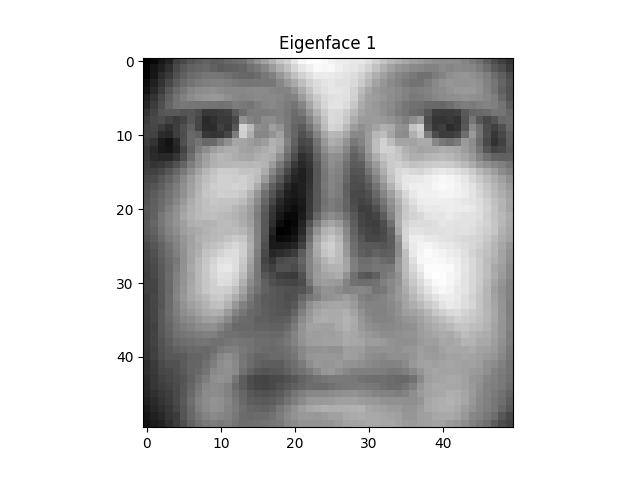
\includegraphics[width=\textwidth]{eigen1.png}
            \caption{Eigenface 1}
        \end{subfigure}
        \begin{subfigure}{0.4\textwidth}
            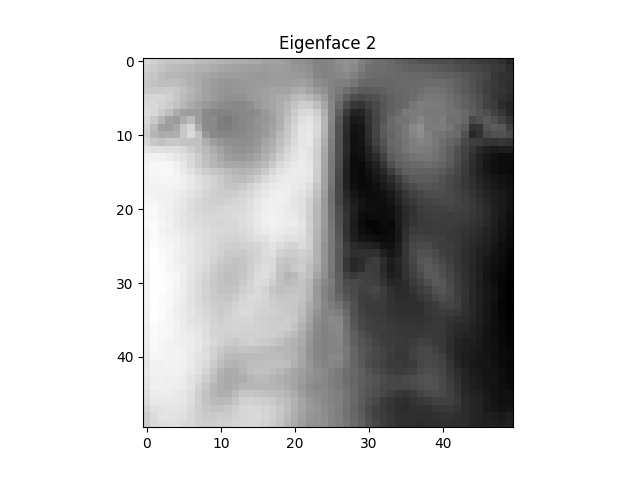
\includegraphics[width=\textwidth]{eigen2.png}
            \caption{Eigenface 2}
        \end{subfigure}
        \begin{subfigure}{0.4\textwidth}
            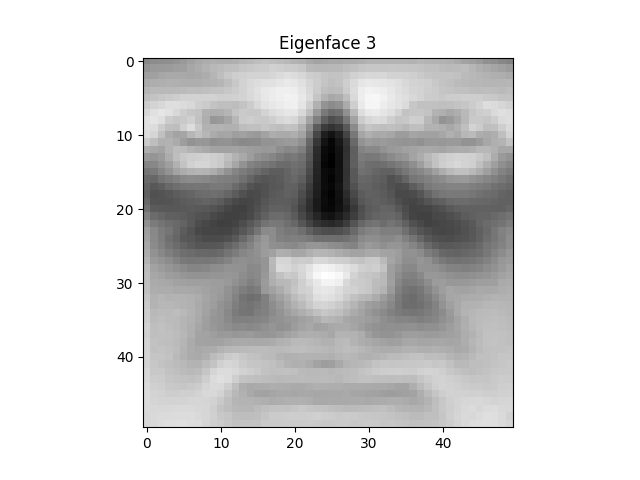
\includegraphics[width=\textwidth]{eigen3.png}
            \caption{Eigenface 3}
        \end{subfigure}
        \begin{subfigure}{0.4\textwidth}
            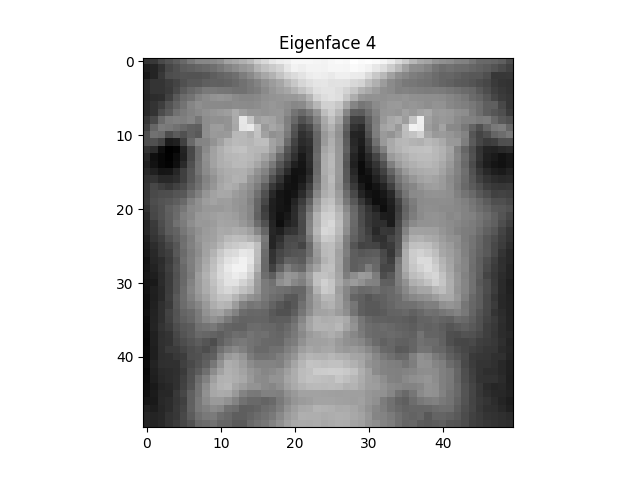
\includegraphics[width=\textwidth]{eigen4.png}
            \caption{Eigenface 4}
        \end{subfigure}
        \begin{subfigure}{0.4\textwidth}
            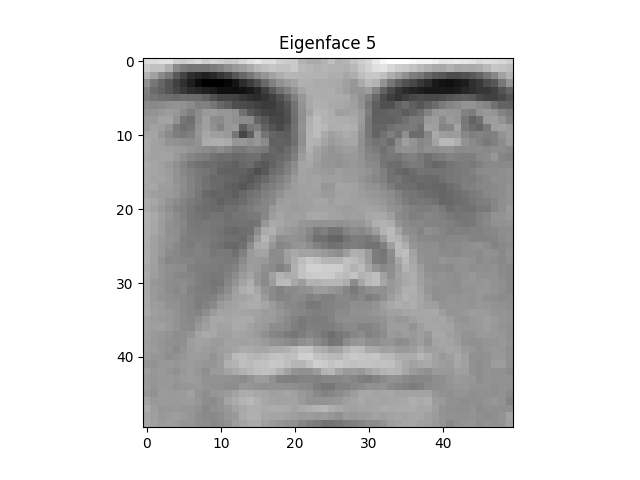
\includegraphics[width=\textwidth]{eigen5.png}
            \caption{Eigenface 5}
        \end{subfigure}
        \caption*{Top 5 Eigenfaces}
        \label{fig:eigenfaces}
    \end{figure}
\end{enumerate}


\clearpage

\section{Thompson Sampling [25 points]}

Consider the Thompson Sampling (TS) algorithm, a Bayesian approach to the multi-armed bandit problem. Consider a Bernoulli bandit with $n$ arms, where each arm $i$ at time-step $1 \leq t \leq T$ has Bernoulli i.i.d rewards $r_{i,t} \in \{0, 1\}$ with $\mathbb{E}[r_{i,t}] = \mu_i$. The TS algorithm starts with a prior distribution of $\mu_i$ for each arm $i$ using the $P_{i,0} \sim \text{Beta}(1, 1)$ distribution and proceeds by selecting an arm based on the posterior distribution as follows. Note the prior distribution of $\mu_i$ at time $t$ is denoted as $P_{i,t-1}$ and the posterior as $P_{i,t}$. Further, the posterior of the current time-step becomes the prior for the next time-step.

\begin{algorithm}[H]
\caption{Thompson Sampling}
\begin{algorithmic}[1]
\For{$t = 1, 2, \ldots, T$}
    \State Sample $\hat{\mu}_{i,t} \sim P_{i,t-1}$ for each arm $i \in \{1, \ldots, n\}$
    \State Play arm $i_t = \arg \max_i \hat{\mu}_{i,t}$
    \State Observe reward $r_{i_t,t}$ and update posterior $P_{i,t}$
\EndFor
\end{algorithmic}
\end{algorithm}

Recall the probability density function of the Beta distribution, $\text{Beta}(\alpha, \beta)$, for any $x \in [0, 1]$ is
\[
p(x) = \frac{(\alpha + \beta - 1)!}{(\alpha - 1)!(\beta - 1)!} x^{\alpha-1} (1 - x)^{\beta-1}.
\]
We also know, for any $p, q \geq 1$,
\[
\int_0^1 x^p (1 - x)^q dx = \frac{(p + q + 1)!}{(p - 1)!(q - 1)!}.
\]

\begin{enumerate}[label=(\alph*)]
    \item Until time-step $t$, suppose arm $i \in \{1, \ldots, n\}$ is pulled $N_{i,t}$ times and its total observed reward is $S_{i,t} := \sum_{u \leq t: i_u = i} r_{i,u}$ where $i_t$ represents the arm chosen at time-step $t$. Find $P_{i,t}$, the posterior distribution of $\mu_i$, given the Beta prior as described above and observations on the rewards until time-step $t$. (Hint: Compute the posterior for the first time-step. Use this recursively for the following time-steps.)
    \subsubsection*{Solution}
    From the Beta distribution, we first define the posterior for the first pull.
    By Bayes rule, the posterior is proportional to the prior times the likelihood:
    \[
    P(\mu_i) \propto P(\mu_i) p(r_{i,1} | \mu_i).
    \]
    The prior is:
    \[
    P(\mu_i) = \text{Beta}(\alpha_{i,0}, \beta_{i,0}) = \text{Beta}(1, 1).
    \]
    Therefore the likelihood of the observed data is:
    \[
    p(data | \mu_i) \propto \mu_i^{S_{i,t}} (1 - \mu_i)^{N_{i,t} - S_{i,t}}.
    \]
    This is proportional to:
    \[
    \mu_i^{S_{i,t}+ 1 -1} (1 - \mu_i)^{N_{i,t} - S_{i,t} + 1 - 1} 
    \]

    This is the Beta distribution with parameters:
    \[
    \alpha_{i,t} = S_{i,t} + 1, \quad \beta_{i,t} = N_{i,t} - S_{i,t} + 1.
    \]

    Therefore the posterior distribution is:
    \[
    P_{i,t}(\mu_i) \approx \text{Beta}(S_{i,t} + 1, N_{i,t} - S_{i,t} + 1).
    \]



    % \begin{align*}
    % P_{i,t}(\mu_i) &\propto P_{i,t-1}(\mu_i) \prod_{u \leq t: i_u = i} p(r_{i,u} | \mu_i) \\
    % &\propto \text{Beta}(\alpha_{i,t-1}, \beta_{i,t-1}) \prod_{u \leq t: i_u = i} \mu_i^{r_{i,u}} (1 - \mu_i)^{1 - r_{i,u}} \\
    % &\propto \mu_i^{\alpha_{i,t-1} - 1} (1 - \mu_i)^{\beta_{i,t-1} - 1} \prod_{u \leq t: i_u = i} \mu_i^{r_{i,u}} (1 - \mu_i)^{1 - r_{i,u}} \\
    % &\propto \mu_i^{\alpha_{i,t-1} - 1 + S_{i,t}} (1 - \mu_i)^{\beta_{i,t-1} - 1 + N_{i,t} - S_{i,t}}.
    % \end{align*}

    % Thus, the posterior distribution is:
    % \[
    % P_{i,t}(\mu_i) = \text{Beta}(\alpha_{i,t}, \beta_{i,t}),
    % \]
    % where
    % \[
    % \alpha_{i,t} = \alpha_{i,t-1} + S_{i,t}, \quad \beta_{i,t} = \beta_{i,t-1} + N_{i,t} - S_{i,t}.
    % \]
    \item Compute the mean and variance of the posterior distribution of $\mu_i$ found in part (a).
    \subsubsection*{Solution}

    \begin{align*}
    \text{Mean} &= \mathbb{E}[\mu_i] = \frac{\alpha_{i,t}}{\alpha_{i,t} + \beta_{i,t}}, \\
    \text{Variance} &= \text{Var}[\mu_i] = \frac{\alpha_{i,t} \beta_{i,t}}{(\alpha_{i,t} + \beta_{i,t})^2 (\alpha_{i,t} + \beta_{i,t} + 1)}.
    \end{align*}

    For the posterior distribution $P_{i,t}(\mu_i) = \text{Beta}(S_{i,t} + 1, N_{i,t} - S_{i,t} + 1)$, we have:
    \[
    Mean = \frac{S_{i,t} + 1}{N_{i,t} + 2}
    \]
    \[
    Variance = \frac{(S_{i,t} + 1)(N_{i,t} - S_{i,t} + 1)}{(N_{i,t} + 2)^2 (N_{i,t} + 3)}.
    \]

    \item Using the computations in part (b), explain how TS balances exploration and exploitation.
    \subsubsection*{Solution}
    Thompson sampling achieves balances between exploration and exploitation through its Bayesian approach. this is how it work
    \begin{itemize}
        \item \textbf{Exploration}: TS samples from the posterior distribution of each arm's reward probability. This sampling introduces randomness, allowing the algorithm to explore arms with high uncertainty. Arms that have not been pulled often or have uncertain reward distributions are more likely to be selected, promoting exploration.
        \item \textbf{Exploitation}: As more data is collected, the posterior distribution becomes more concentrated around the true reward probabilities. The mean of the posterior distribution, which represents the expected reward for each arm, guides the algorithm towards arms that have historically provided higher rewards. This leads to exploitation of the best-performing arms.
        \item \textbf{Dynamic Balance}: The balance between exploration and exploitation is dynamic. Initially, when the algorithm has limited information about the arms, it explores more. As time progresses and more data is collected, the algorithm shifts towards exploitation, focusing on the arms that have shown higher rewards. This natural transition occurs without explicit tuning of parameters.
        \item \textbf{Posterior Variance}: The variance of the posterior distribution quantifies the uncertainty in the estimate of the reward probabilities. Arms with higher variance are more likely to be explored, while arms with lower variance are exploited. This ensures that the algorithm continues to explore even after some arms have been identified as good choices.
        \item \textbf{Thompson Sampling's Efficiency}: TS efficiently balances exploration and exploitation by leveraging the posterior distribution of the reward probabilities. The mean of the posterior distribution represents the expected reward for each arm based on observed data. The variance quantifies the uncertainty in this estimate. By sampling from the posterior, TS naturally incorporates both exploration and exploitation into its decision-making process.
    \end{itemize}
    % Thompson Sampling balances exploration and exploitation by leveraging the posterior distribution of the reward probabilities for each arm. The mean of the posterior distribution, $\mathbb{E}[\mu_i] = \frac{\alpha_{i,t}}{\alpha_{i,t} + \beta_{i,t}}$, represents the expected reward for arm $i$ based on observed data. The variance, $\text{Var}[\mu_i] = \frac{\alpha_{i,t} \beta_{i,t}}{(\alpha_{i,t} + \beta_{i,t})^2 (\alpha_{i,t} + \beta_{i,t} + 1)}$, quantifies the uncertainty in this estimate.

    % During each time-step, TS samples $\hat{\mu}_{i,t}$ from the posterior distribution $P_{i,t-1}$. This sampling introduces randomness, allowing the algorithm to occasionally select arms with high uncertainty (exploration) rather than always choosing the arm with the highest mean reward (exploitation). Over time, as more data is collected, the variance of the posterior distribution decreases, leading to more confident estimates of $\mu_i$ and a natural shift toward exploitation. This dynamic ensures that TS efficiently balances exploration and exploitation without requiring explicit tuning of parameters.
\end{enumerate}



\clearpage

\section{Gridworld [25 points]}

Consider the following grid environment. Starting from any unshaded square, you can move up, down, left, or right. Actions are deterministic and always succeed (e.g., going left from state 16 goes to state 15) unless they will cause the agent to run into a wall. The thicker edges indicate walls, and attempting to move in the direction of a wall results in staying in the same square (e.g., going in any direction other than left from state 16 stays in 16). Taking any action from the target square with cheese (no. 11) earns a reward of $r_g$ (so $r(11, a) = r_g \, \forall a$) and ends the episode. Taking any action from the square of the cat (no. 6) earns a reward of $r_r$ (so $r(6, a) = r_r \, \forall a$) and ends the episode. Otherwise, from every other square, taking any action is associated with a reward $r_s \in \{-1, 0, +1\}$ (even if the action results in the agent staying in the same square). Assume the discount factor $\gamma = 1$, $r_g = +10$, and $r_r = -1000$ unless otherwise specified.

\begin{figure}[H]
    \centering
    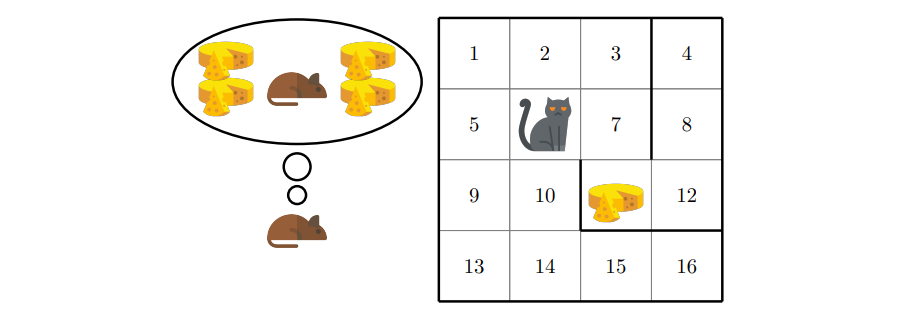
\includegraphics[width=0.6\textwidth]{gridworld.png}
    \caption{Gridworld environment}
    \label{fig:gridworld}
\end{figure}

\begin{enumerate}[label=(\alph*)]
    \item \textbf{Policy Evaluation [9 points]} \\
    Let $r_s = 0$. In the policy below, the arrow in each box denotes the (deterministic) action that should be taken in each state. Evaluate the following policy and show the corresponding value (i.e., cumulative reward) for every state (square).

    \[
    \begin{array}{|c|c|c|c|}
    \hline
    \rightarrow & \rightarrow & \downarrow & \downarrow \\ \hline
    \rightarrow & \rightarrow & \downarrow & \downarrow \\ \hline
    \uparrow & \uparrow & \downarrow & \leftarrow \\ \hline
    \uparrow & \uparrow & \leftarrow & \leftarrow \\ \hline
    \end{array}
    \]

    \subsubsection*{Solution}
    % \subsubsection*{Solution}
    To evaluate the given policy, we compute the value of each state using the Bellman equation for policy evaluation. Since \( r_s = 0 \), the reward for each step is zero except for the terminal states (cheese and cat). The value of a state is the expected cumulative reward starting from that state and following the policy.

    Let \( V(s) \) denote the value of state \( s \). For non-terminal states, the value is computed as:
    \[
    V(s) = r_s + \gamma V(s'),
    \]
    where \( s' \) is the next state determined by the policy.

    For terminal states:
    \[
    V(11) = r_g = 10, \quad V(6) = r_r = -1000.
    \]

    % Using \( \gamma = 1 \), we iteratively compute the values for all states until convergence. The resulting values are:

    \textbf{Values for each state:}
    \begin{enumerate}
        \item State 1: $\rightarrow 2 \rightarrow 3 \downarrow 7 \downarrow 11$ = cheese(+10)
        \item State 2: $\rightarrow 3 \downarrow 7 \downarrow 11$ = cheese(+10)
        \item State 3: $\downarrow 7 \downarrow 11$ = cheese(+10)
        \item State 4: $\downarrow 8 \downarrow 12 \leftarrow 11$ = cheese(+10)
        \item State 5: $\rightarrow 6$ = cat(-1000)
        \item State 6: cat(-1000)
        \item State 7: $\downarrow 11$ = cheese(+10)
        \item State 8: $\downarrow 12 \leftarrow 11$ = cheese(+10)
        \item State 9: $\uparrow 5 \leftarrow 6$ = cat(-1000)
        \item State 10: $\uparrow 6$ = cat(-1000)
        \item State 11: cheese(+10)
        \item State 12: $\leftarrow 11$ = cheese(+10)
        \item State 13: $\uparrow 9 \uparrow 5 \rightarrow 6$ = cat(-1000)
        \item State 14: $\uparrow 10 \uparrow 6$ = cat(-1000)
        \item State 15: $\leftarrow 14 \uparrow 10 \uparrow 6 $ = cat(-1000)
        \item State 16: $\leftarrow 15 \leftarrow 14 \uparrow 10 \uparrow 6$ = cat(-1000)
    \end{enumerate}

    Therefore the values for each state are as follows:
    \[
    \begin{array}{|c|c|c|c|}
    \hline
    10 & 10 & 10 & 10 \\ \hline
    -1000 & -1000 & 10 & 10 \\ \hline
    -1000 & -1000 & 10 & 10 \\ \hline
    -1000 & -1000 & -1000 & -1000 \\ \hline
    \end{array}
    \]

    % \[
    % \begin{array}{|c|c|c|c|}
    % \hline
    % -6 & -5 & -4 & -3 \\ \hline
    % -5 & -4 & -3 & -2 \\ \hline
    % -4 & -3 & -2 & -1 \\ \hline
    % -3 & -2 & -1 & 0 \\ \hline
    % \end{array}
    % \]

    These values represent the cumulative reward for each state under the given policy.
    \item \textbf{Optimal Policy with Shortest Path [8 points]} \\
    Define the value of $r_s$ that would cause the optimal policy to return the shortest path to the cheese square (no. 11); note that your value for $r_s$ should lie in $\{-1, 0, +1\}$. Using this $r_s$, find the optimal value for each square and the optimal policy.
    \subsubsection*{Solution}
    \subsubsection*{Solution}
    To determine the optimal policy that returns the shortest path to the cheese square (no. 11), we need to ensure that the agent prioritizes reaching the cheese over any other considerations. This can be achieved by setting \( r_s = -1 \), which penalizes each step taken, encouraging the agent to minimize the number of steps.

    % Using \( r_s = -1 \), the optimal value for each square and the corresponding optimal policy are computed using dynamic programming or value iteration. The resulting optimal policy and values are as follows:

    We will use Bellman optimal equation which is:
    \[
    V*s = \max_a \left( r_s + \gamma \sum_{s'} P(s'|s, a)V^*(s') \right)
    \]
    Since $\gamma  = 1$ this simplifies it to:
    \[
    V*(s) = \max_a \left( r_s + \sum_{s'} P(s'|s, a)V^*(s') \right)
    \]

    % State 6 and 11 are terminal states with $V*(6)=-1000 and V*(11)=10.$
    \textbf{Terminal States:}
    \begin{itemize}
        \item \( V^*(6) = -1000 \) (cat square)
        \item \( V^*(11) = 10 \) (cheese square)
    \end{itemize}

    \textbf{One step from the cheese square:}
    \begin{itemize}
        \item \( V^*(7) = 10 - 1 = 9 \) (action $\downarrow$)
        \item \( V^*(12) = 10 - 1 = 9 \) (action $\leftarrow$)
    \end{itemize}

    \textbf{Two steps from the cheese square:}
    \begin{itemize}
        \item \( V^*(3) = 9 - 1 = 8 \) (action $\downarrow 7$)
        \item \( V^*(8) = 9 - 1 = 8 \) (action $\downarrow 12$)
    \end{itemize}

    \textbf{Three steps from the cheese square:}
    \begin{itemize}
        \item \( V^*(2) = 8 - 1 = 7 \) (action $\rightarrow 3$)
        \item \( V^*(4) = 8 - 1 = 7 \) (action $\downarrow 8$)
    \end{itemize}

    \textbf{Four steps from the cheese square:}
    \begin{itemize}
        \item \( V^*(1) = 7 - 1 = 6 \) (action $\rightarrow 2$)
    \end{itemize}

    \textbf{Five steps from the cheese square:}
    \begin{itemize}
        \item \( V^*(5) = 6 - 1 = 5 \) (action $\uparrow 1$)
    \end{itemize}

    \textbf{Six steps from the cheese square:}
    \begin{itemize}
        \item \( V^*(9) = 5 - 1 = 4 \) (action $\uparrow 5$)
    \end{itemize}

    \textbf{Seven steps from the cheese square:}
    \begin{itemize}
        \item \( V^*(10) = 4 - 1 = 3 \) (action $\leftarrow 9$)
        \item \( V^*(13) = 4 - 1 = 3 \) (action $\uparrow 9$)
    \end{itemize}

    \textbf{Eight steps from the cheese square:}
    \begin{itemize}
        \item \( V^*(14) = 3 - 1 = 2 \) (action $\uparrow 10$)
    \end{itemize}

    \textbf{Nine steps from the cheese square:}
    \begin{itemize}
        \item \( V^*(15) = 2 - 1 = 1 \) (action $\leftarrow 14$)
    \end{itemize}

    \textbf{Ten steps from the cheese square:}
    \begin{itemize}
        \item \( V^*(16) = 1 - 1 = 0 \) (action $\leftarrow 15$)
    \end{itemize}


    The optimal values for each state are as follows:
    \[
    \begin{array}{|c|c|c|c|}
    \hline
    6 & 7 & 8 & 7 \\ \hline
    5 & -1000 & 9 & 8 \\ \hline
    4 & 3 & 10 & 9 \\ \hline
    3 & 2 & 1 & 0 \\ \hline
    \end{array}
    \]

    \text{bf Optimal Policy:}
    \[
    \begin{array}{|c|c|c|c|}
    \hline
    \rightarrow & \rightarrow & \downarrow & \downarrow \\ \hline
    \uparrow & T & \downarrow & \downarrow \\ \hline
    \uparrow & \leftarrow & T & \leftarrow \\ \hline
    \uparrow & \uparrow & \leftarrow & \leftarrow \\ \hline
    \end{array}
    \]


    % \[
    % \text{Optimal Policy:}
    % \begin{array}{|c|c|c|c|}
    % \hline
    % \rightarrow & \rightarrow & \downarrow & \downarrow \\ \hline
    % \rightarrow & \rightarrow & \downarrow & \downarrow \\ \hline
    % \rightarrow & \rightarrow & \downarrow & \leftarrow \\ \hline
    % \rightarrow & \rightarrow & \leftarrow & \leftarrow \\ \hline
    % \end{array}
    % \]

    % \[
    % \text{Optimal Values:}
    % \begin{array}{|c|c|c|c|}
    % \hline
    % -6 & -5 & -4 & -3 \\ \hline
    % -5 & -4 & -3 & -2 \\ \hline
    % -4 & -3 & -2 & -1 \\ \hline
    % -3 & -2 & -1 & 0 \\ \hline
    % \end{array}
    % \]

    % Here, the values represent the cumulative reward (negative due to \( r_s = -1 \)) for each square under the optimal policy, with the shortest path to the cheese square being prioritized.

    \item \textbf{Effect of Adding +2 to All Rewards [8 points]} \\
    Let’s refer to the value function derived in part (b) as \( V^\pi_{g,\text{old}} \), and the policy as \( \pi_g \). Suppose we are now in a new gridworld where all the rewards (\( r_s \), \( r_g \), and \( r_r \)) have \( +2 \) added to them. Consider still following the policy \( \pi_g \), which is optimal for the original gridworld. What will the new value function \( V^\pi_{g,\text{new}} \) be in this second gridworld?
    \subsubsection*{Solution}
    \begin{align*}
    V^\pi_{g,\text{new}}(s) &= V^\pi_{g,\text{old}}(s) + \frac{2}{1 - \gamma},
    \end{align*}
    The new rewards are:
    \begin{itemize}
        \item \( r_s = -1 + 2 = 1 \)
        \item \( r_g = 10 + 2 = 12 \)
        \item \( r_r = -1000 + 2 = -998 \)
    \end{itemize}

    The new value function \( V^\pi_{g,\text{new}} \) can be expressed as:
    \[
    V^\pi_{g,\text{new}}(s) = V^\pi_{g,\text{old}}(s) + \frac{2}{1 - \gamma} = V^\pi_{g,\text{old}}(s) + 2.
    \]

    This means that the new value function is simply the old value function plus a constant offset of 2 for all states. The optimal policy remains unchanged, but the values are shifted uniformly.

    \textbf{Terminal States:}
    \begin{itemize}
        \item \( V^\pi_{g,\text{new}}(6) = -998 \) (cat square)
        \item \( V^\pi_{g,\text{new}}(11) = 12 \) (cheese square)
    \end{itemize}

    \textbf{State by state values:}
    \begin{itemize}
        \item State 7: 7$\downarrow 11$ = 1 + 12 = 13
        \item State 12: 12$\leftarrow 11$ = 1 + 12 = 13
        \item State 3: 3$\downarrow 7$ = 1 + 13 = 14
        \item State 8: 8$\downarrow 12$ = 1 + 13 = 14
        \item State 2: 2$\rightarrow 3$ = 1 + 14 = 15
        \item State 4: 4$\downarrow 8$ = 1 + 14 = 15
        \item State 1: 1$\rightarrow 2$ = 1 + 15 = 16
        \item State 5: 5$\uparrow 1$ = 1 + 16 = 17
        \item State 9: 9$\uparrow 5$ = 1 + 17 = 18
        \item State 10: 10$\leftarrow 9$ = 1 + 18 = 19
        \item State 13: 13$\uparrow 9$ = 1 + 18 = 19
        \item State 14: 14$\uparrow 10$ = 1 + 19 = 20
        \item State 15: 15$\leftarrow 14$ = 1 + 20 = 21
        \item State 16: 16$\leftarrow 15$ = 1 + 21 = 22
    \end{itemize}

    The new values for each state are as follows:
    \[
    \begin{array}{|c|c|c|c|}
    \hline
    16 & 15 & 14 & 15 \\ \hline
    17 & -998 & 13 & 14 \\ \hline
    18 & 19 & 12 & 13 \\ \hline
    19 & 20 & 21 & 22 \\ \hline
    \end{array}
    \]
    % \[
    % \text{The new value function is:}
    % \begin{array}{|c|c|c|c|}
    % \hline
    % 8 & 9 & 10 & 9 \\ \hline
    % 7 & -998 & 11 & 10 \\ \hline
    % 6 & 5 & 12 & 11 \\ \hline
    % 5 & 4 & 3 & 2 \\ \hline
    % \end{array}
    % \]
\end{enumerate}




\clearpage

\section{[Bonus] Markov Decision Process as Linear Program [20 points]}

(This question is optional and counts towards extra credit.)

Consider a Markov Decision Process (MDP) \( M = \{S, A, P, r, \gamma\} \) where \( S \) is the state space, \( A \) is the action space, \( P \) is the transition kernel representing the probability of transition to state \( s' \) from state \( s \) when action \( a \) is taken as \( P(s'|s, a) \), \( r \) is the reward function and \( \gamma \) is the discount factor. Consider the linear program

\[
\min_{V \in \mathbb{R}^{|S|}} \sum_{s \in S} \rho(s)V(s)
\]
\[
\text{s.t. } V(s) \geq r(s, a) + \gamma \sum_{s' \in S} P(s'|s, a)V(s') \quad \forall s \in S, a \in A
\]

where \( \rho(s) \in \mathbb{R}_+ \, \forall s \in S \) and denote its solution as \( V^\star \in \mathbb{R}^{|S|} \).

\begin{enumerate}[label=(\alph*)]
    \item Show that the dual formulation of the above linear program can be written as
    \[
    \max_{x \in \mathbb{R}^{|S \times A|}} \sum_{s \in S, a \in A} r(s, a)x(s, a)
    \]
    \[
    \text{s.t. } \sum_{a \in A} x(s, a) - \gamma \sum_{s' \in S, a' \in A} P(s|s', a')x(s', a') = \rho(s) \quad \forall s \in S
    \]
    \[
    x(s, a) \geq 0 \quad \forall s \in S, a \in A.
    \]

    \subsubsection*{Solution}
    To derive the dual formulation, we start with the primal linear program:

    \[
    \min_{V \in \mathbb{R}^{|S|}} \sum_{s \in S} \rho(s)V(s)
    \]
    \[
    \text{s.t. } V(s) \geq r(s, a) + \gamma \sum_{s' \in S} P(s'|s, a)V(s') \quad \forall s \in S, a \in A.
    \]

    % Step 1: Write the constraints in standard form
    The inequality constraints can be rewritten as:
    \[
    r(s, a) + \gamma \sum_{s' \in S} P(s'|s, a)V(s') - V(s) \leq 0 \quad \forall s \in S, a \in A.
    \]

    % ### Step 2: Formulate the Lagrangian
    Introduce dual variables \( x(s, a) \geq 0 \) for each constraint. The Lagrangian is:
    \[
    L(V, x) = \sum_{s \in S} \rho(s)V(s) + \sum_{s \in S} \sum_{a \in A} x(s, a) \left( r(s, a) + \gamma \sum_{s' \in S} P(s'|s, a)V(s') - V(s) \right).
    \]

    % ### Step 3: Simplify the Lagrangian
    Reorganize terms in the Lagrangian:
    \[
    L(V, x) = \sum_{s \in S} \rho(s)V(s) + \sum_{s \in S} \sum_{a \in A} x(s, a)r(s, a) + \gamma \sum_{s \in S} \sum_{a \in A} \sum_{s' \in S} x(s, a)P(s'|s, a)V(s') - \sum_{s \in S} \sum_{a \in A} x(s, a)V(s).
    \]

    Combine terms involving \( V(s) \):
    \[
    L(V, x) = \sum_{s \in S} \left( \rho(s) - \sum_{a \in A} x(s, a) + \gamma \sum_{s' \in S} \sum_{a' \in A} x(s', a')P(s|s', a') \right)V(s) + \sum_{s \in S} \sum_{a \in A} x(s, a)r(s, a).
    \]

    % ### Step 4: Dual problem
    The dual function is obtained by minimizing \( L(V, x) \) with respect to \( V \). For the dual to be bounded below, the coefficient of \( V(s) \) must equal zero:
    \[
    \rho(s) - \sum_{a \in A} x(s, a) + \gamma \sum_{s' \in S} \sum_{a' \in A} x(s', a')P(s|s', a') = 0 \quad \forall s \in S.
    \]

    The dual objective is:
    \[
    \max_{x \geq 0} \sum_{s \in S} \sum_{a \in A} x(s, a)r(s, a).
    \]

    Thus, the dual problem is:
    \[
    \max_{x \in \mathbb{R}^{|S \times A|}} \sum_{s \in S, a \in A} r(s, a)x(s, a)
    \]
    \[
    \text{s.t. } \sum_{a \in A} x(s, a) - \gamma \sum_{s' \in S, a' \in A} P(s|s', a')x(s', a') = \rho(s) \quad \forall s \in S,
    \]
    \[
    x(s, a) \geq 0 \quad \forall s \in S, a \in A.
    \]

    \item Denote the optimal solution to the dual problem as \( x^\star \in \mathbb{R}^{|S \times A|} \). Due to strong duality and complementary slackness, we have
    \[
    x^\star(s, a) \left( V^\star(s) - \gamma \sum_{s' \in S} P(s'|s, a)V^\star(s') - r(s, a) \right) = 0 \quad \forall s \in S, a \in A.
    \]
    Now, show that the optimal policy \( \pi^\star(\cdot|s), \forall s \in S \), can be derived as
    \[
    \pi^\star(a|s) =
    \begin{cases}
    1 & \text{if } a = \arg \max_{a \in A} x^\star(s, a) \\
    0 & \text{else.}
    \end{cases}
    \]

    \subsubsection*{Solution}
    To derive the optimal policy \( \pi^\star(\cdot|s) \), we use the complementary slackness condition:
    \[
    x^\star(s, a) \left( V^\star(s) - \gamma \sum_{s' \in S} P(s'|s, a)V^\star(s') - r(s, a) \right) = 0 \quad \forall s \in S, a \in A.
    \]

    This implies that for \( x^\star(s, a) > 0 \), the term in parentheses must equal zero:
    \[
    V^\star(s) = \gamma \sum_{s' \in S} P(s'|s, a)V^\star(s') + r(s, a).
    \]

    Thus, the optimal value \( V^\star(s) \) is achieved by selecting the action \( a \) that maximizes the right-hand side:
    \[
    a^\star = \arg \max_{a \in A} \left( r(s, a) + \gamma \sum_{s' \in S} P(s'|s, a)V^\star(s') \right).
    \]

    Since \( x^\star(s, a) > 0 \) only for the optimal action \( a^\star \), the optimal policy \( \pi^\star(\cdot|s) \) is given by:
    \[
    \pi^\star(a|s) =
    \begin{cases}
    1 & \text{if } a = \arg \max_{a \in A} x^\star(s, a), \\
    0 & \text{otherwise.}
    \end{cases}
    \]
\end{enumerate}

\end{document}